\chapter{Arquitetura}

A arquitetura foi pensada para ser implementada com o Docker e Docker Compose. Cada
programa que precisa ser executado é rodado em um serviço separado. Exceto o Gunicorn,
todos os outros serviços usam imagens prontas do Docker Hub, o que oferece mais segurança
com as atualizações constantes.

\begin{figure}[ht]
    \begin{center}
    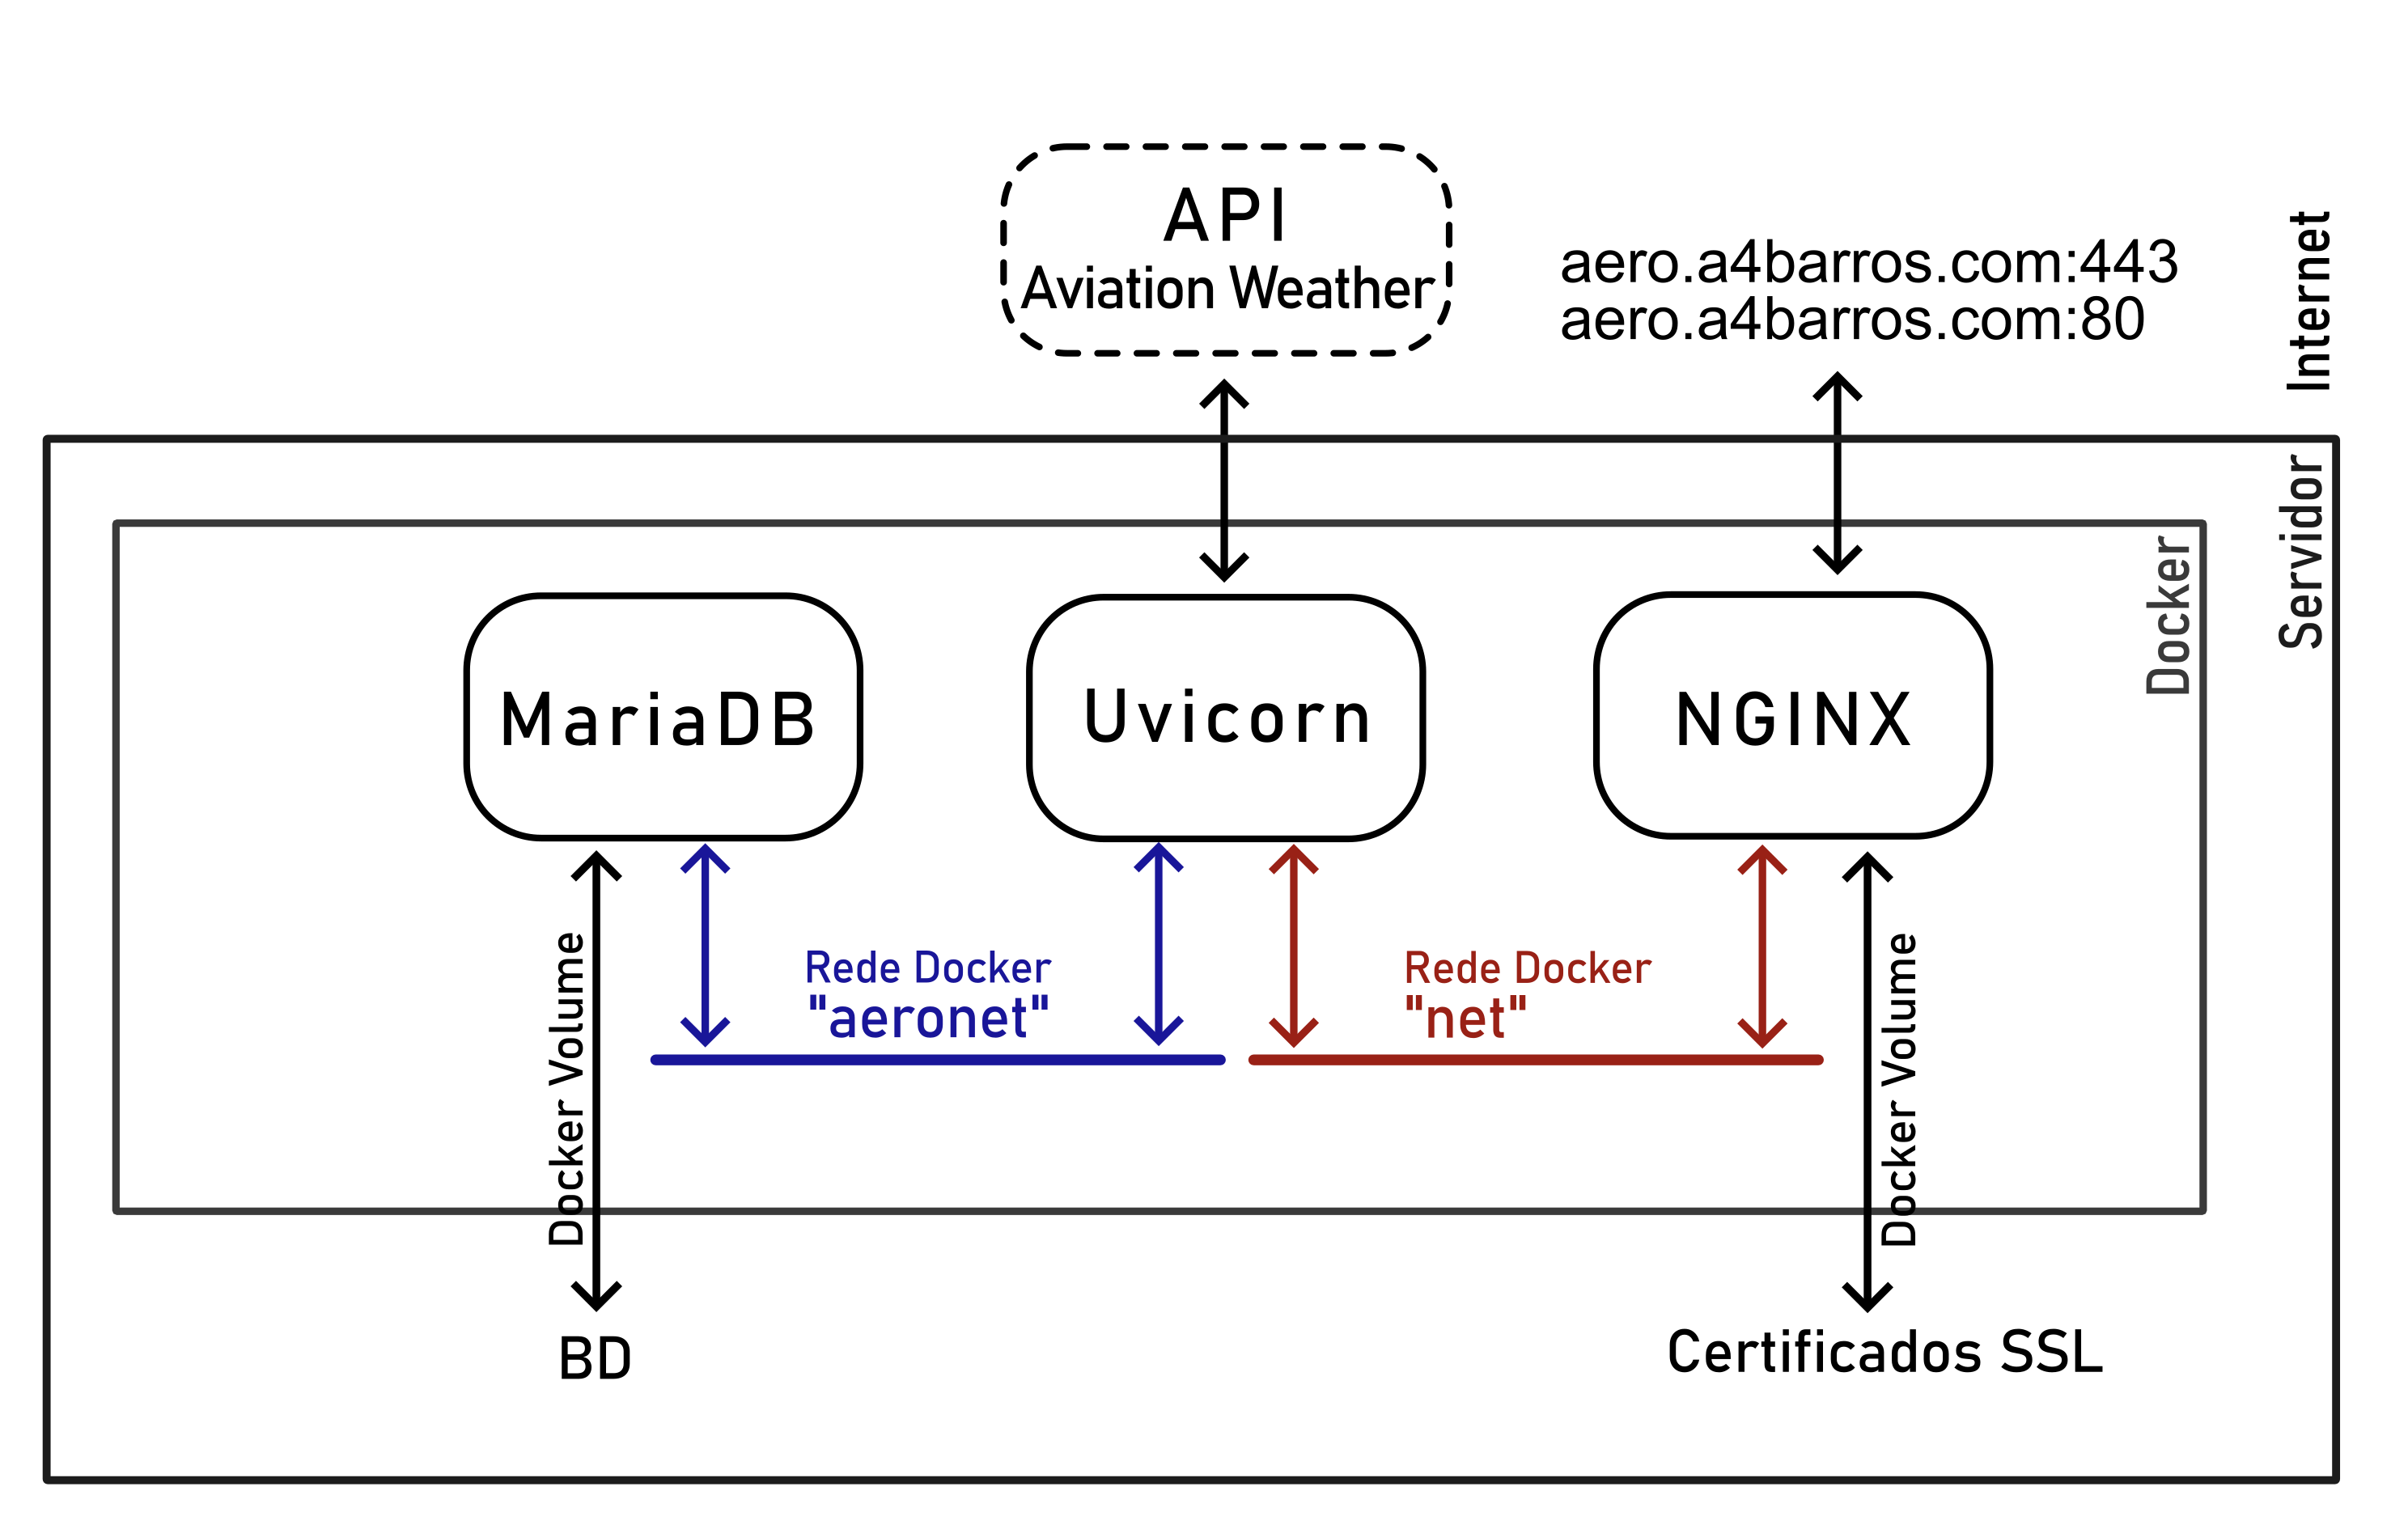
\includegraphics[width=\linewidth]{img/diagrama-arquitetura.png}
    \caption{Modelo de Arquitetura}
    \label{fig:arquitetura}
    \end{center}
\end{figure}

\section{Docker Network}
A porta 5000 do Gunicorn não estará disponível para todos os serviços. Por segurança, é usada a função de
"network". Observe no diagrama que a proxy NGINX compartilha com o Gunicorn a rede "net", para o NGINX,
o Gunicorn não pode ser acessado por \texttt{localhost:5000}, e sim por \texttt{http://aero:5000}, "aero"
sendo o nome do serviço no Docker Compose.


\section{Docker Secrets}

Para aumentar a segurança de acesso ao banco, é usada a funcionalidade "secrets". Nela, no Docker Compose,
você informa um arquivo de texto no host onde estará uma senha, uma senha por arquivo. No mesmo Compose,
você informa quais serviços têm acesso a cada senha. Caso o serviço de banco de dados, por exemplo, tenha
acesso a senha db-password.txt, será feito um bind do arquivo db-password.txt no host para o "/run/secret/db-password.txt"
no guest.
Tanto os bancos como o servidor Gunicorn usam este método para terem acesso às senhas dos bancos.

\section{Serviços}

\subsection{MariaDB}
Este banco de dados relacional guarda toda a informação mais ou menos fixa sobre os aeródromos,
conforme explicado no capítulo de modelo de dados.

\section{FastAPI}

O site foi construído com a framework FastAPI tanto para desenvolvimento quanto para produção, 
utilizando o servidor embutido do FastAPI, o Uvicorn.

Diferentemente do Flask, em que era necessário usar um servidor externo (o Gunicorn no caso 
deste projeto), o servidor do FastAPI (Uvicorn \cite{uvicorn}), com a configuração padrão, é 
suficiente para produção. Usando o comando \texttt{uvicorn server:app --host 0.0.0.0 --port 5000}, 
o servidor é iniciado em modo de produção.

\subsection{Proxy NGINX}
O NGINX faz o HTTPS funcionar, dá suporte ao HTTP/2 e ao cabeçalho HTTP keep-alive. Quando
utilizava o Gunicorn, ele só tinha suporte ao primeiro, e a documentação do Gunicorn não
recomendava que ele estivesse diretamente ligado à Internet \cite{nginx-gunicorn}. O Uvicorn,
no momento em que este texto foi escrito, não suporta HTTP/2, mas suporta o keep-alive. No
entanto, como tenho outros projetos na mesma máquina, utilizo subdomínios. Todos os subdomínios
resolvem para a mesmo IP/máquina via "A RECORD", mas na configuração
do NGINX, o bloco de servidor com o hostname aero.a4barros.com é redirecionado para o
endereço interno "http://aero:5000".

\section{Produção}
O site se encontra em produção no endereço https://aero.a4barros.com. Ele está hospedado em uma VPS
da Oracle Cloud Infrastructure com as seguintes características de hardware:

\begin{itemize}
    \item \textbf{CPU:} AMD EPYC 7551 (2 cores) @ 1.996GHz
    \item \textbf{RAM:} 1GB
    \item \textbf{Armazenamento:} 25GB
    \item \textbf{SO:} Ubuntu 22.04.4 LTS
\end{itemize}

\begin{figure}[ht]
    \begin{center}
    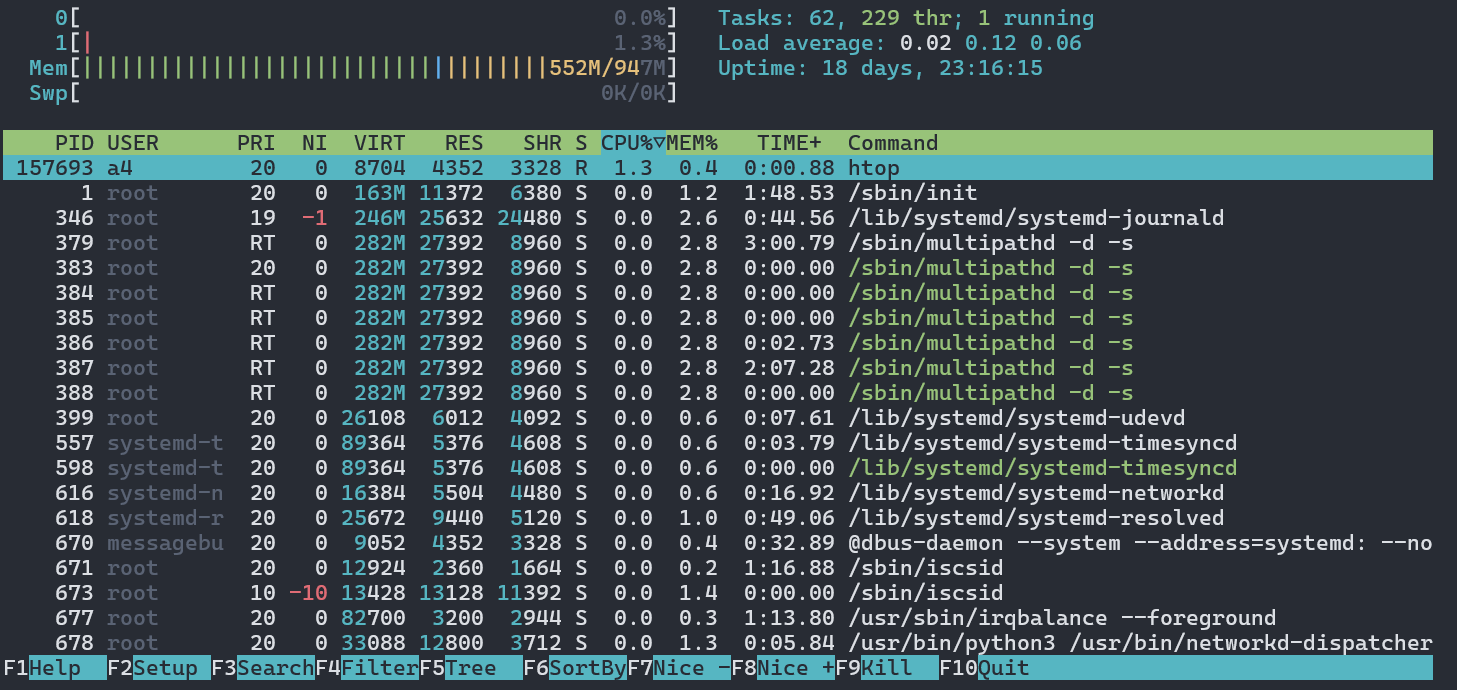
\includegraphics[width=400pt]{img/prod-idle.png}
    \caption{Uso do sistema em baixa demanda}
    \label{fig:prod-idle}
    \end{center}
\end{figure}

Mesmo com uma configuração bastante modesta, o sistema roda sete containers Docker, usando 
aproximadamente metade da memória primária (RAM) em idle.

\begin{figure}[ht]
    \begin{center}
    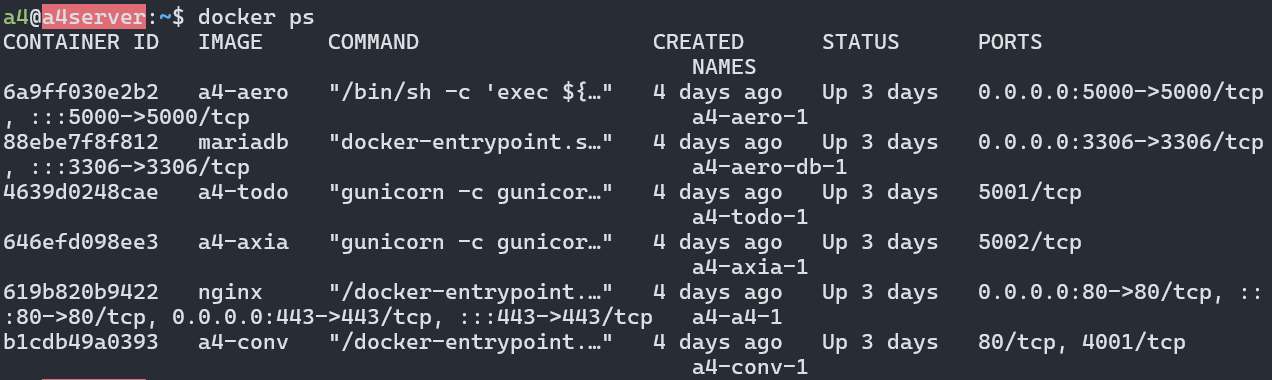
\includegraphics[width=400pt]{img/containers.png}
    \caption{Containers Docker em execução}
    \label{fig:containers}
    \end{center}
\end{figure}

\section{Diagrama de sequência}

\begin{figure}[ht]
    \begin{center}
    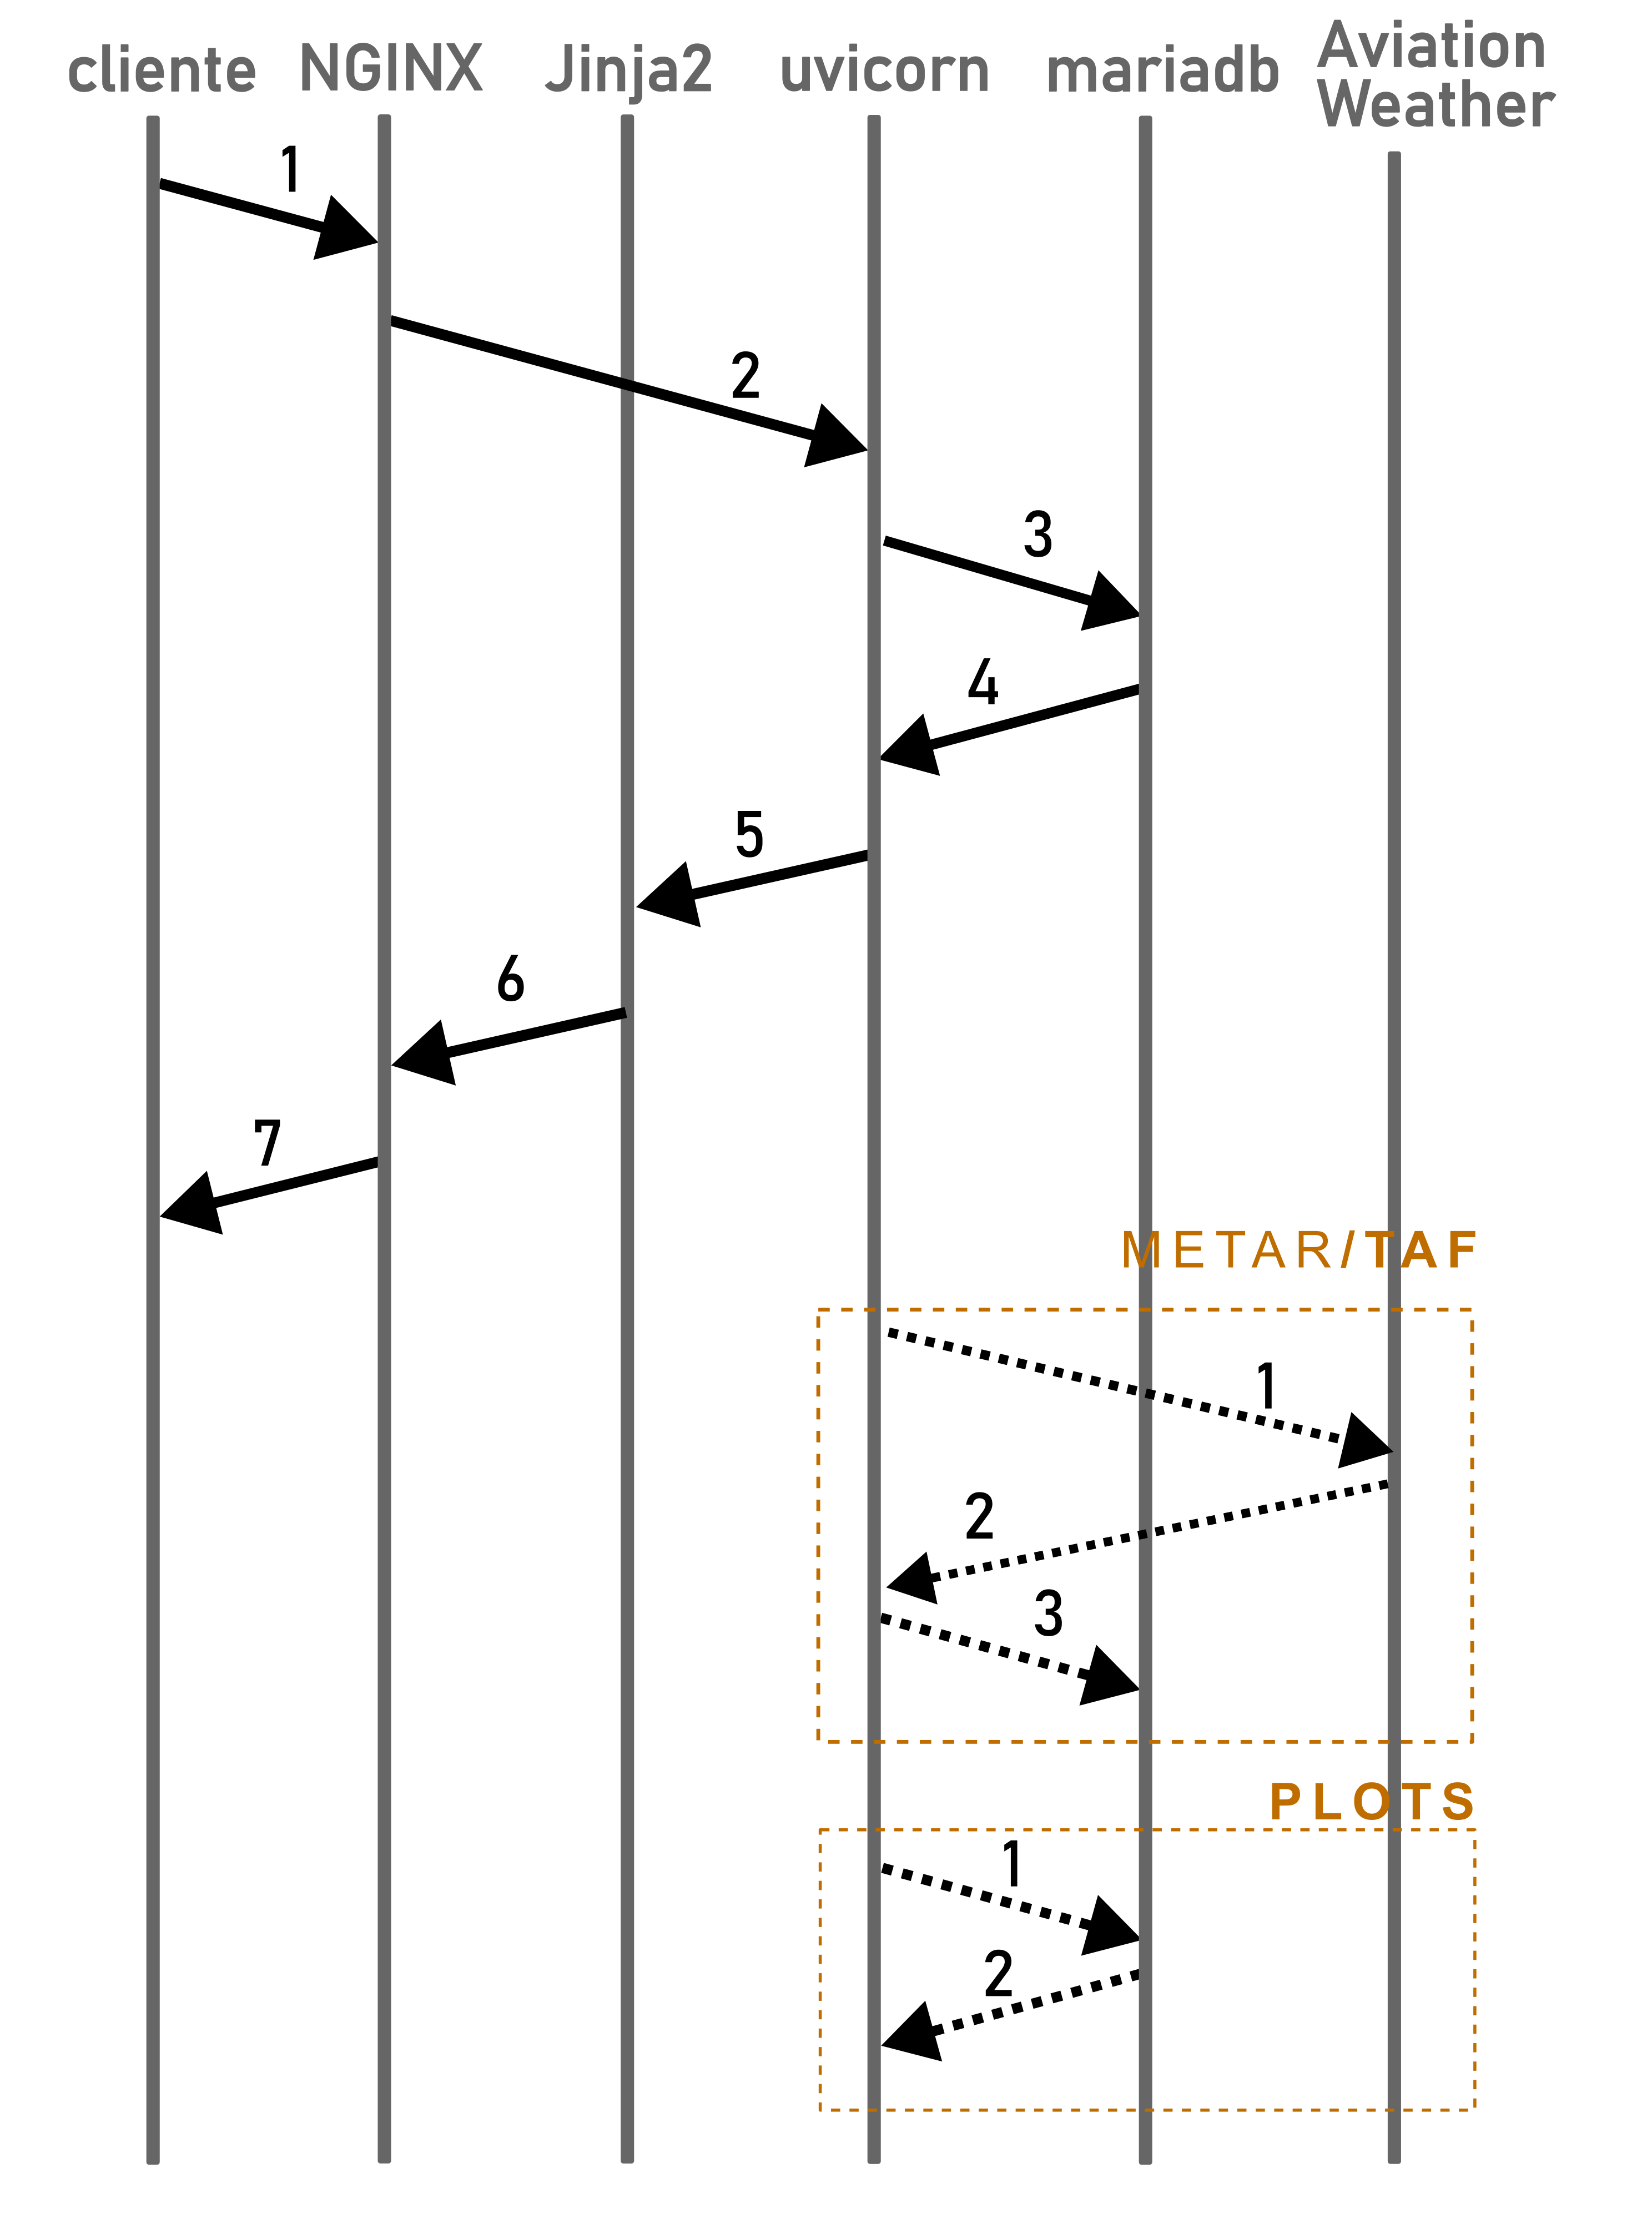
\includegraphics[width=0.5\linewidth]{img/diagrama-tempo.png}
    \caption{Diagrama de sequência}
    \label{fig:tempo}
    \end{center}
\end{figure}

\begin{enumerate}
\item O usuário realiza uma requisição para a rota raiz ou "/info/\{icao\}".
\item Um servidor NGINX funcionando como proxy realiza o limite de requisições por segundo
e bloqueia user-agents que aparentem ser robôs. Caso a requisição passe pelo filtro, é
realizado um proxy-pass para o servidor Gunicorn.
\item Para a rota raiz, é feito um SELECT no banco para pegar informações de todos os
aeroportos. Na rota "/info/\{icao\}", é feito um SELECT-WHERE para buscar apenas um aeroporto.
A ORM é usada para isto, portanto os comandos SQL não aparecem diretamente no código.
\item O banco de dados responde à requisição. Para a rota "/info/\{icao\}", é verificado 
se o METAR existente no banco é válido para aquela hora. Se for, o sistema vai para o passo 8;
se não, continua para o passo 5.
\item É feita uma requisição para a API do Aviation Weather pedindo o METAR para o 
aeroporto em questão. O sistema vai para o passo 3.
\item A API responde.
\item O METAR atualizado é gravado no banco.
\item O servidor envia as informações necessárias ao Jinja2 para a geração da página.
\item A página HTML é gerada.
\item O usuário recebe esta página.
\end{enumerate}
